\subsection{Loop interchange}
If we inline the function \textbf{value} into the main loop we get what Figure
\ref{fig:inline_value} shows.

\begin{figure}[!ht]
	\centering
		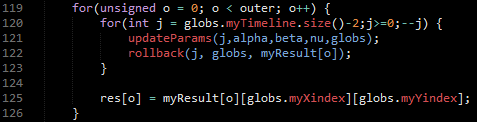
\includegraphics[scale=0.8]{input/figures/inline_value.png}
		\caption{The main loop where \textbf{value} is inlined.\label{fig:inline_value}}
\end{figure}

We can see that we can perform loop distribution on the inner loop and the
write to \emph{res}. By doing so, we are now able to loopinterchange the two
outer loops calling \textbf{updateParams} and \textbf{rollback} as we can see in
Figure \ref{fig:main_loopinterchange}.

\begin{figure}[!ht]
	\centering
		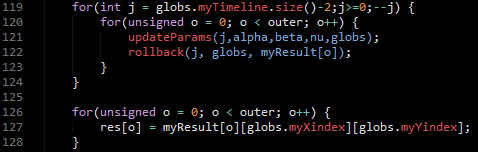
\includegraphics[scale=0.8]{input/figures/main_loopinterchange.png}
		\caption{The main loop where a loopinterchange has been performed.\label{fig:main_loopinterchange}}
\end{figure}

Our loopinterchange is safe since the loop over \emph{outer} is parallel.
The final loop, writing to \emph{res} is translated into the
\textbf{buildResultKernel} kernel in the CUDA version.
We note that \textbf{updateParams} is constant across all iterations of
\emph{outer} and hence it can be extracted out of the loop. If we then inline
\textbf{updateParams} we get a loopnest that is ready to become a kernel.
This code transformation can be seen in Figure \ref{fig:inline_updateparams}.

\begin{figure}[!ht]
	\centering
		\includegraphics[scale=0.75]{input/figures/inline_updateparams.png}
		\caption{The main loop where \textbf{updateParams} is inlined.\label{fig:inline_updateparams}}
\end{figure}

It makes it more clear that the inlined
code is parallelized for a CUDA kernel, as there are no cross iteration
dependencies and is translated into the \textbf{myVarXYKernel} kernel in our
CUDA version. We note that part of the computation is constant across each
iteration of the two inner dimensions.
